\documentclass[12pt]{article}
\usepackage[utf8]{inputenc}

% Importing settings from setup.sty
\usepackage{setup}
\usepackage{booktabs}
\usepackage{multicol}
\usepackage{multirow}
\usepackage{glossaries}
% \makenoidxglossaries
\newcommand{\prox}{\operatorname{prox}}

% \newacronym{bmi}{BMI}{Body Mass Index}


% \pagenumbering{roman}
\begin{document}

% Inserting title page
\import{./}{title}

\pagenumbering{gobble}
\tableofcontents
% \listoffigures
% \listoftables



\newgeometry{
  left=25mm,
  right=25mm,
  top=25mm,
  bottom=25mm}
\pagenumbering{arabic}

\section{Thread model: Deploy models}
\subsection{Understanding the attack}
\subsubsection{Level of information of the attacker}
The attacker has access to the global model only, as can be seen in the function:
\begin{align*}
              & \texttt{attacker.py}              \\
  \rightarrow & \texttt{Attacker}                 \\
  \rightarrow & \texttt{model\_inversion\_attack}
\end{align*}
which only takes as argument the global model (\texttt{model}) and the number of rounds (\texttt{nb\_rounds}).

\subsubsection{What is a model inversion attack?}
A model inversion attack, also called gradient inversion attack, is an attack that aims at recovering the training dataset from the global model. This is the attack that the attacker performs in our case.

\subsection{Getting familiar with the dataset}
\subsubsection{Plot one image}
% TODO: plot one image

\subsubsection{Name of the data heterogeneity}
In this case, each of the $N = 10$ client holds one image of each of the 40 subjects. The data distribution for each client is \textbf{homogeneous}. This is to be opposed to the case where the data distribution would be splitted by labels, \eg the case $N = 40$ where each client holds 10 image of only one subject.

\subsection{Evaluating the performance of the attack}
\subsubsection{Precise notation for the SSIM metric.}
The SSIM metric represents the similarity between two images. It uses the following elements:
\begin{enumerate}
  \item $\mu_x$ is the mean of the image $x$.
  \item $\mu_y$ is the mean of the image $y$.
  \item $\sigma_x$ is the standard deviation of the image $x$.
  \item $\sigma_y$ is the standard deviation of the image $y$.
  \item $\sigma_{xy}$ is the covariance between the images $x$ and $y$.
  \item $L$ is the dynamic range of the images.
  \item $k_1$ and $k_2$ are two constants that stabilize the division when the denominator is close to zero. They are set to $k_1 = 0.01$ and $k_2 = 0.03$ from the \href{https://ece.uwaterloo.ca/~z70wang/publications/ssim.pdf}{original paper}
  \item $c_1 = (k_1 L)^2$ and $c_2 = (k_2 L)^2$ are two constants that depend on the dynamic range of the images. They stabilize the division when the denominator is close to zero.
\end{enumerate}
The SSIM metric is defined as:
\begin{equation}
  \text{SSIM}(x, y) = \frac{(2 \mu_x \mu_y + c_1)(2 \sigma_{xy} + c_2)}{(\mu_x^2 + \mu_y^2 + c_1)(\sigma_x^2 + \sigma_y^2 + c_2)}
\end{equation}
The SSIM ranges between $-1$ and $1$. The closer to $1$, the more similar the two images are. The closer to $-1$, the more different the two images are. It can be interpreted as a correlation coefficient.

\subsection{Exercise 1}
Table \ref{tab:SSIM} shows the SSIM for various values of $\alpha$ and local steps $E$. $\alpha$ represent how much the local model is IID. Larger values of $\alpha$ means that the local model is more IID.
% make a table with the SSIM for various values of alpha
% put alpha on the columns and E on the rows
\begin{table}[h]
  \centering
  \begin{tabular}{c|c|c|c|c}
            & $\alpha = 0.1$ & 0.5   & 0.7   \\ \hline
    $E = 1$ & 0.018          & 0.017 & 0.017 \\
    10      & 0.025          & 0.022 & 0.023 \\
    20      & 0.025          & 0.023 & 0.024 \\
    50      & 0.027          & 0.024 & 0.026 \\
  \end{tabular}
  \caption{SSIM for various values of the non-IID coefficient $\alpha$ and the local steps $E$.}
  \label{tab:SSIM}
\end{table}
We see that for a given number of local steps $E$, the SSIM increases as $\alpha$ increases. This means that the more the local model is IID, the better the global model is.

% the more you increase alpha, the more you are IID
\section{Thread model: Honest-but-curious server}
\subsection{Exercise 2}
We run the experiment with the attack occurring at various number of rounds. The results are shown in Figure \ref{fig:SSIM}.
\begin{figure}[h]
  \centering
  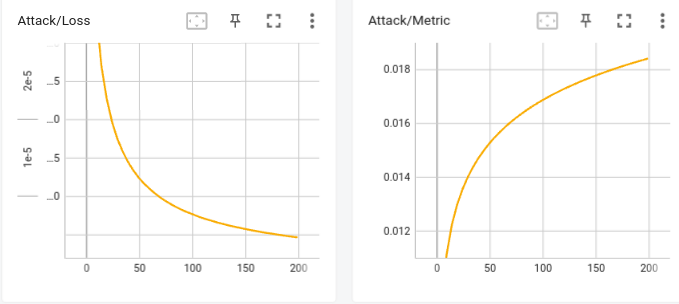
\includegraphics[width=0.8\textwidth]{./images/ssim_200.png}
  \caption{SSIM and attack loss for various values number of rounds}
  \label{fig:SSIM}
\end{figure}
We see that the SSIM increases as time passes and the attack loss decreases. This means that it is better for the attacker to perform the attack at the end of the training. This is because the global model is better at the end of the training. It has already learnt a well-performing model so it is easier for the attacker to recover the training dataset. \\
This conclusion actually makes sense as the initial model is not trained at all (pretty much random) so it is harder for the attacker to recover the training dataset.

% \clearpage
% \printnoidxglossaries

\end{document}